%________________________________________________________________________________________________

\chapter{Introduction}

In the world we live in, concurrency is ubiquitous. Imagine that we are walking inside a forest. Different birds, animals and insects are talking around us. Suddenly we see a beautiful bird peeping from a branch of a sunlit mossy tree. Our brain here is processing multiple sensory information, motor control, and cognition concurrently. Visual cortex is processing images while auditory cortex is processing sounds. Motor cortex is controlling movement while cerebellum is maintaining balance. Hippocampus is forming memories while prefrontal cortex maybe making a decision whether to capture this moment in our camera or not. At the same time, autonomic nervous system is regulating heart rate and breathing. And at this moment if a mosquito bites our hand, the hand moves automatically spoiling the camera image, as it is being controlled by spinal cord reflexes which is operating independently of our conscious brain control.

In nature, truly sequential systems are rare. Cellular processes, ecosystem dynamics, flocking, schooling and colony behaviour etc. all happen concurrently. However, they are more common when manmade artifacts are considered. In particular, computer systems are often developed from a sequential perspective. However, the need for increasingly powerful, flexible and usable automated systems has become mainstream, which has made concurrency unavoidable. 

Most such concurrent systems are also time-critical. We see examples of such systems everyday in automotive systems, where the collision avoidance system processes camera data every 33ms for example, and radar data every 50ms. All sensors work concurrently but must fuse their data within a 10ms window for brake activation. In Pacemakers, where multiple concurrent processes monitor heart rhythm, detect arrhythmias, and deliver electrical impulses, all with microsecond timing precision. The sensing circuit operates at a different rate while the pacing circuit has variable timing based on heart rate. In 5G telecommunications networks, multiple radio frequency channels operate concurrently, and handles thousands of concurrent user connections while maintaining precise timing synchronization. In a manufacturing assembly line multiple robotic arms must coordinate their movements within microsecond precision. Each arm operates concurrently but must synchronize at specific timed intervals to avoid collisions.

In time-critical concurrent systems, even a minor malfunction can have catastrophic consequences, leading to significant loss of life or financial devastation. This inherent risk underscores the crucial need for rigorous verification to ensure these systems operate flawlessly at all times. In essence, ensuring their correct behavior is paramount to maintaining the smooth functioning of our society. This highlights the practical imperative behind the formal study of concurrent systems . Formal verification, a specialized research area, provides automated algorithmic solutions to mathematically guarantee the correct behavior of systems. The theoretical motivation lies in developing mathematical theories for new areas of interest. 

Although concurrent systems are common in our world, no mathematical theory of concurrent systems existed until the pioneering work of Carl Petri \cite{} in the 1960s. In the theory of sequential computation various mathematical models have been proposed in the last several decades, e.g., Turing machines \cite{}, the $\lambda$-calculus \cite{}, etc. For concurrent computation, however, an agreement on how to formally represent the observable behaviour of a concurrent or distributed system does not exist yet, and consequently, the model of concurrency is still to be developed. Negotiations \cite{} is one of the newest such models, which has been proposed as a concurrency primitive. Timed automata \cite{} is a popular formalism, amenable to verification, used in situations where the systems we want to model have associated temporal constraints. It is very natural to model timed-concurrent systems as timed-negotiations \cite{}, which operate concurrently for different processes and synchronize on joint actions.

Formal verification is one of the most active research area within theoretical computer science. It deals with the problem where given a system $S$ and a specification $spec$ (which could be safety specification) does the behaviour of the system satisfy the specification, i.e., $S \models spec$? Reachability analysis involves determining whether a system can transition from a given initial state to a specified target state or set of states. Reachability analysis is an integral part of verification. To verify a system, we first need to analyze its reachability to determine if it can even reach the states required by the specification. For instance, in safety verification, you would first need to determine if the system can reach any unsafe states. If it can't, then the safety specification is satisfied. 

In timed-concurrent systems, the enormous state-space presents a significant challenge for reachability analysis, often leading to computationally expensive state-space exploration. Therefore, the scalability of algorithmic solutions is paramount, alongside their correctness and efficiency. Partial order reduction \cite{} (POR) techniques aim to address this "state-space explosion" by systematically reducing the search space explored during verification. However, the effectiveness of POR hinges on accurately determining the independence of actions. While this is straightforward in untimed systems, the implicit synchronization imposed by time in timed systems complicates independence computations, especially within networks of timed automata. This difficulty forms the primary hurdle in extending POR to networks of timed automata. 

This thesis focuses on tackling the reachability problem within a novel model of timed-concurrent systems: local-timed negotiations, which offer a promising avenue for applying POR techniques.
%__________________________________________________________________________________

\section{Negotiations, timed automata,\\ and reachability}

Our problem of interest for this thesis is \textit{location reachability problem for local-timed negotiations}. In this section we discuss reachability problem in timed automata and negotiations with examples. We will discuss local time semantics in Chapter \ref{}.

\subsection{Reachability problem for timed automata}

A timed automaton \cite{} is a finite state automaton augmented with a set of non-negative real-valued variables called \textit{clock}. The clocks are initially set to zero and increase at the same rate along with time. Clocks are used to constraint the transitions, i.e., the transitions of the automaton are associated with a conjunction of inequalities which compares a clock variable to a natural number, referred to as \textit{guards}. This represents that the transition can be taken only when the value of the clocks satisfies the guard associated with the transition. Additionally, some clocks can be \textit{reset} (i.e., their values can be set to $0$) on taking a transition. The reset operation allows to measure time intervals between events. just like in finite state automata, a timed automaton also has an initial state and a set of accepting states. Figure ~\ref{fig:ab} gives an example of a timed automaton with clocks $\{x, y\}$, with initial state $q_0$ and accepting state $q_2$, over the alphabet $\{a, b\}$.

\begin{figure}[t]
\centering
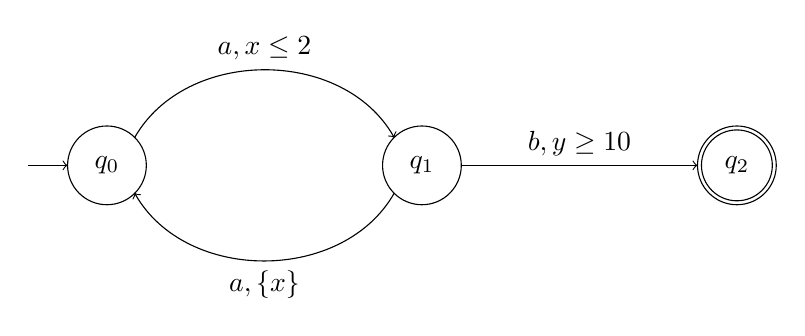
\begin{tikzpicture}[scale=1, every node/.style={transform shape}]

\filldraw [fill=white]  (0,0)  circle (5mm) node (q0) {$q_0$};
\filldraw [fill=white]  (4,0)  circle (5mm) node (q1) {$q_1$};
\filldraw [fill=white]  (8,0)  circle (5mm) node (q2) {$q_2$};
\draw (8,0)  circle (4.5mm);

\begin{scope}[->]
\draw (0.35,0.35) .. controls (1,1.5) and (3,1.5) .. (3.65,0.35) node [midway, above] {$a, x \leq 2$};
\draw (3.65,-0.35) .. controls (3,-1.5) and (1,-1.5) .. (0.35,-0.35) node [midway, below] {$a, \{x\}$};
\draw (4.5,0) -- (7.5,0) node [midway, above] {$b, y \geq 10$};
\draw (-1,0) -- (-0.5,0);
\end{scope}

\end{tikzpicture}
\caption{A timed automaton $\calA_1$. Both the clocks $x$ and $y$ start together at $q_0$. The transition on $a$ from state $q_0$ to $q_1$ has a guard on the clock $x$, which forces to spend at most $2$ units of time before taking the transition. The transition on the letter $a$ from $q_1$ to $q_0$ can be taken without any time constraint. $\{x\}$ denotes that the clock $x$ is reset while taking the transition on the letter $a$. The guard on the letter $b$ says that the total time spent must be at least $10$ units of time before the accepting state $q_2$ can be reached.}
\label{fig:ab}
\end{figure}

A fundamental problem arising in the study of timed automata is the \textit{reachability problem}. The reachability problem for a timed automaton asks if there exists a run of the automaton from an initial state to an accepting state. This is useful in checking if some bad state of a system could possibly be reached. Verification algorithms for timed automata have been widely studied and are the basis for a number of verification tools such as TChecker \cite{}, UPPAAL \cite{}, KRONOS \cite{}, Theta \cite{} etc.

\begin{figure}[t]
\centering
\begin{tikzpicture}

\node at (0,0) {$(q_0, \langle 0, 0 \rangle)$};
\node at (-4,-2) {$(q_1, \langle 0, 0 \rangle)$};
\node at (0,-2) {$(q_1, \langle 0.8, 0.8 \rangle)$};
\node at (4,-2) {$(q_1, \langle 1.5, 1.5 \rangle)$};
\node at (-4,-4) {$(q_0, \langle 0, 0.8 \rangle)$};
\node at (0,-4) {$(q_0, \langle 0, 5.8 \rangle)$};
\node at (4,-4) {$(q_0, \langle 0, 9.8 \rangle)$};
\node at (0,-6) {$(q_1, \langle 0.5, 10.3 \rangle)$};
\node at (4,-6) {$(q_1, \langle 1.2, 11 \rangle)$};
\node at (8,-6) {$(q_1, \langle 1.8, 11.6  \rangle)$};
\node at (4,-8) {$(q_2, \langle 2.2, 12 \rangle)$};

\node at (-2,-2) {$\cdots$};
\node at (2,-2) {$\cdots$};
\node at (6,-2) {$\cdots$};
\node at (-2,-4) {$\cdots$};
\node at (2,-4) {$\cdots$};
\node at (6,-4) {$\cdots$};
\node at (-2,-6) {$\cdots$};
\node at (2,-6) {$\cdots$};
\node at (6,-6) {$\cdots$};
\node at (10,-6) {$\cdots$};
\node at (2,-8) {$\cdots$};
\node at (6,-8) {$\cdots$};
\node at (-4,-2.5) {$\vdots$};
\node at (4,-2.5) {$\vdots$};
\node at (-4,-4.5) {$\vdots$};
\node at (0,-4.5) {$\vdots$};
\node at (0,-6.5) {$\vdots$};
\node at (8,-6.5) {$\vdots$};

\begin{scope}[-Stealth]
\draw (0,-0.3) -- (-4,-1.7) node [midway, left, above] {\footnotesize $0$};
\draw (0,-0.3) -- (0,-1.7) node [midway, left] {\footnotesize $0.8$};
\draw (0,-0.3) -- (4,-1.7) node [midway, right, above] {\footnotesize $1.5$};
\draw (0,-2.3) -- (-4,-3.7) node [midway, left, above] {\footnotesize $0$};
\draw (0,-2.3) -- (0,-3.7) node [midway, left] {\footnotesize $5$};
\draw (0,-2.3) -- (4,-3.7) node [midway, right, above] {\footnotesize $9$};
\draw (4,-4.3) -- (0,-5.7) node [midway, left, above] {\footnotesize $0.5$};
\draw (4,-4.3) -- (4,-5.7) node [midway, left] {\footnotesize $1.2$};
\draw (4,-4.3) -- (8,-5.7) node [midway, right, above] {\footnotesize $1.8$};
\draw (4,-6.3) -- (4,-7.7) node [midway, left] {\footnotesize $1$};
\end{scope}

\end{tikzpicture}
\caption{Part of the transition system showing the behaviours of the timed automaton $\calA_1$}
	\label{fig:ab-behavior}
\end{figure}

Figure ~\ref{} shows a part of the transition system showing the behaviours of the timed automaton Figure ~\ref{}. Starting from the initial state $q_0$ and the initial clock valuation $\langle 0, 0 \rangle$, which means $x = 0, y = 0$, the automaton can choose to spend any amount of time between $0$ to $2$ units to reach the state $q_1$. So, if $0.8$ time units are spent at $q_0$, the valuation becomes $\langle 0.8, y = 0.8 \rangle$. The automaton can spend an arbitrary amount of time (say $9$ units) at $q_1$ if it wants to take the $a$ transition. After taking the transition on the letter $a$ where $x$ is reset, the clock valuation becomes $\langle 0, 9.8 \rangle$ and the automaton goes back to $q_0$. Spending $1.2$ time units at $q_0$ and taking the $a$ transition to $q_1$ the valuation becomes $\langle 11, 1.2 \rangle$. Now the guard on $b$ can be satisfied and after spending an arbitrary amount of time at $q_1$ the final state $q_2$ can be reached.

As we see, the space of configurations is uncountably infinite as the clocks takes values from the set of positive real numbers. To solve the reachability problem, one needs to know if there is a sequence of enabled transitions leading to the final state. To know if a transition is enabled, one needs to check if the values of clocks before taking the transition satisfy the corresponding guard. For any fixed sequence of transitions in the underlying DFA, we have uncountably many executions of the timed automaton, where each execution differs from the other in the assignment to the clock variables (valuations) in at least one of the steps of the execution. This calls for an effective and efficient handling of the uncountably infinite space of clock valuations. This is the main challenge faced in the reachability analysis.

The first solution to the reachability problem goes by a partition of the space of clock valuations into a finite number of abstractions called \textit{regions} \cite{}, such that all valuations in a region becomes indistinguishable by the timed automaton with respect to state reachability. The definition of regions is parameterised by a bound function $M$ that associates to every clock $x$ the maximum constant appearing in a guard involving $x$. For example, the maximum bounds function $M_1$ for the automaton $\calA_1$ assigns $M_1(x) = 2$, and $M_1(y) = 10$. The maximum bounds function also ensures finiteness of the number of regions. Once the space of valuations is partitioned into this finite number of regions, a cross product with the states of the automaton is taken to give what is called the region graph. It has been proved that the region graph is sound and complete for state reachability \cite{}. While this gives an effective solution to the reachability problem for timed automata, however, in practice, it turns out that the region graphs are too large to be of use for efficiently checking the reachability of timed automata.

The most widely used approach for reachability analysis in timed automata relies on the concept of \textit{zones} \cite{}. These are convex sets defined by constraints involving only the differences between clocks. Zones offer a significant advantage due to their efficient representation and manipulation using Difference Bound Matrices (DBMs) \cite{}, leading to efficient algorithms \cite{}. However, for the purposes of this thesis, we work only with regions.

\subsection{Reachability problem for local-timed negotiations}

Before describing local-timed negotiations and the reachability problem in this model, introducing the underlying negotiation model with an example is necessary, which we discuss next.

\subsubsection{Negotiations}

A multiparty \textit{atomic negotiation} involves the synchronized action of several \textit{processes} (\textit{agents}) to jointly select an outcome from a finite set. In \cite{} Esparza and Desel introduced \textit{distributed negotiations} (or simply \textit{negotiations}) as a model of concurrency using these multiparty atomic interactions as primitive. This model structures a workflow of atomic negotiations where, after each atomic negotiation, participating agents collaboratively agree on an outcome and proceed to a subsequent set of atomic negotiations, as defined by the workflow.

\begin{figure}[t]
\centering
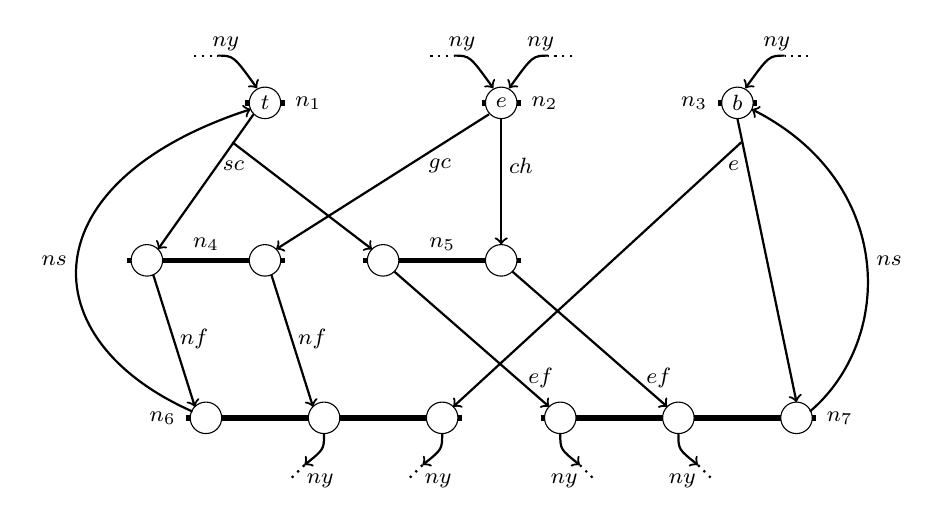
\begin{tikzpicture}[scale=1, every node/.style={transform shape}]

\begin{scope}[line width=2pt]
\draw (-0.25,0) -- (0.25,0);
\draw (2.75,0) -- (3.25,0);
\draw (5.75,0) -- (6.25,0);
\draw (-1.75,-2) -- (0.25,-2);
\draw (1.25,-2) -- (3.25,-2);
\draw (-1,-4) -- (2.5,-4);
\draw (3.5,-4) -- (7,-4);
\end{scope}

\filldraw [fill=white]  (0,0)  circle (2mm) node (t0) {\footnotesize $t$};
\filldraw [fill=white]  (3,0)  circle (2mm) node (e0) {\footnotesize $e$};
\filldraw [fill=white]  (6,0)  circle (2mm) node (b0) {\footnotesize $b$};
\filldraw [fill=white]  (-1.5,-2)  circle (2mm) node (t1) {};
\filldraw [fill=white]  (0,-2)  circle (2mm) node (e1) {};
\filldraw [fill=white]  (1.5,-2)  circle (2mm) node (t2) {};
\filldraw [fill=white]  (3,-2)  circle (2mm) node (e2) {};
\filldraw [fill=white]  (-0.75,-4)  circle (2mm) node (t5) {};
\filldraw [fill=white]  (0.75,-4)  circle (2mm) node (e5) {};
\filldraw [fill=white]  (2.25,-4)  circle (2mm) node (b5) {};
\filldraw [fill=white]  (3.75,-4)  circle (2mm) node (t6) {};
\filldraw [fill=white]  (5.25,-4)  circle (2mm) node (e6) {};
\filldraw [fill=white]  (6.75,-4)  circle (2mm) node (b6) {};

\node at (0.55,0) {\footnotesize $n_1$};
\node at (3.55,0) {\footnotesize$n_2$};
\node at (5.45,0) {\footnotesize $n_3$};
\node at (-0.75,-1.8) {\footnotesize $n_4$};
\node at (2.25,-1.8) {\footnotesize $n_5$};
\node at (-1.3,-4) {\footnotesize $n_6$};
\node at (7.3,-4) {\footnotesize $n_7$};

\node at (-0.4, -0.8) {\footnotesize $sc$};
\node at (2.22, -0.8) {\footnotesize $gc$};
\node at (3.25, -0.8) {\footnotesize $ch$};
\node at (5.95, -0.8) {\footnotesize $e$};
\node at (-0.9,-3) {\footnotesize $nf$};
\node at (0.6, -3) {\footnotesize $nf$};
\node at (3.5,-3.5) {\footnotesize $ef$};
\node at (5,-3.5) {\footnotesize $ef$};
\node at (0.7, -4.8) {\footnotesize $ny$};
\node at (2.2, -4.8) {\footnotesize $ny$};
\node at (3.8, -4.8) {\footnotesize $ny$};
\node at (5.3, -4.8) {\footnotesize $ny$};
\node at (-0.5, 0.75) {\footnotesize $ny$};
\node at (2.5, 0.75) {\footnotesize $ny$};
\node at (3.5, 0.75) {\footnotesize $ny$};
\node at (6.5, 0.75) {\footnotesize $ny$};

\begin{scope}[thick,->]
\draw (-0.145, -0.145) -- (-1.36, -1.86); %t0-t1
\draw (-0.415, -0.5) -- (1.36, -1.86); %t0-t2
\draw (2.845, -0.145) -- (0.14, -1.86); %e0-e1
\draw (3, -0.2) -- (3, -1.8); %e0-e2
\draw (-1.5, -2) + (0.08, -0.18) -- (-0.89, -3.86); %t1-t3
\draw (0, -2) + (0.08, -0.18) -- (0.61, -3.86); %e1-e3
\draw (1.5, -2) + (0.145, -0.145) -- (3.61, -3.86); %t2-t4
\draw (3, -2) + (0.145, -0.145) -- (5.11, -3.86); %e2-e4
\draw (6.05, -0.5) -- (2.39, -3.86); %b0-b3
\draw (6, -0.2) -- (6.75, -3.8); %b0-b4
\draw (-0.92, -3.92) .. controls (-3, -3) and (-3, -1) .. (-0.18, -0.08) node [midway, left] {\footnotesize $ns$}; %t3-t0
\draw (6.92, -3.92) .. controls (8, -3) and (8, -1) .. (6.18, -0.08) node [midway, right] {\footnotesize $ns$}; %b4-b0
\draw (0.75,-4.2) .. controls (0.75, -4.4) .. (0.5,-4.6) ; %e3-e0
\draw (2.25, -4.2) .. controls (2.25, -4.4) .. (2, -4.6); %b3-b0
\draw (3.75, -4.2) .. controls (3.75, -4.4) .. (4, -4.6); %t4-t0
\draw (5.25, -4.2) .. controls (5.25, -4.4) .. (5.5, -4.6); %e4-e0
\draw (-0.6, 0.6) .. controls (-0.4, 0.6) .. (-0.1, 0.185); %t4-t0
\draw (2.4, 0.6) .. controls (2.6, 0.6) .. (2.9, 0.185); %e3-e0
\draw (3.6, 0.6) .. controls (3.4, 0.6) .. (3.1, 0.185); %e4-e0
\draw (6.6, 0.6) .. controls (6.4, 0.6) .. (6.1, 0.185); %b3-b0
\end{scope}

\begin{scope}[thick, dotted]
\draw (-0.9, 0.6) -- (-0.6, 0.6);
\draw (2.1, 0.6) -- (2.4, 0.6);
\draw (3.9, 0.6) -- (3.6, 0.6);
\draw (6.9, 0.6) -- (6.6, 0.6);
\draw (0.5,-4.6) -- (0.3, -4.8);
\draw (2, -4.6) -- (1.8, -4.8);
\draw (4, -4.6) -- (4.2, -4.8);
\draw (5.5, -4.6) -- (5.7, -4.8);
\end{scope}

\end{tikzpicture}
\caption{The early flowering of many plants due to climate change is creating a critical synchronization problem for insect pollinators like bees \cite{}. When flowers and their necessary pollinators are out of sync, insects lack food, causing potential disruptions throughout the food web. The above figure provides a simplified diagram of this concurrent phenomenon modelled as incomplete distributed negotiations. $t$, $e$, and $b$ are the agents here, denoting \textit{trees}, \textit{environment}, and \textit{bees}, respectively, participating in the nodes $n_1$, $n_2$, and $n_3$, respectively. $n_1$, $n_2$, and $n_3$ are all nodes with a single \textit{domain}, i.e., only one process participates in these nodes. $n_2$ has two outgoing actions, $gc$ and $ch$, denoting \textit{good climate} and \textit{climate change}. $n_1$ and $n_3$ have outgoing actions $sc$ and $e$ respectively, denoting \textit{season change} and \textit{emergence of bees}. In $n_4$, where $t$ and $e$ participate, $nf$ (\textit{normal flowering}) can take place if $gc$ has taken place previously. Otherwise in $n_5$, $ef$ (\textit{early flowering}) takes place if $ch$ was taken in $n_2$ instead of $gc$. $n_6$ and $n_7$ both have single outgoing action $ny$, denoting \textit{next year}, which takes the three processes back to $n_1$, $n_2$, and $n_3$ (four of these arcs are shown partially for the sake of clarity of the picture).}
	\label{fig:pollination}
\end{figure}

\begin{figure}[t]
\centering
\begin{minipage}{.49\textwidth}
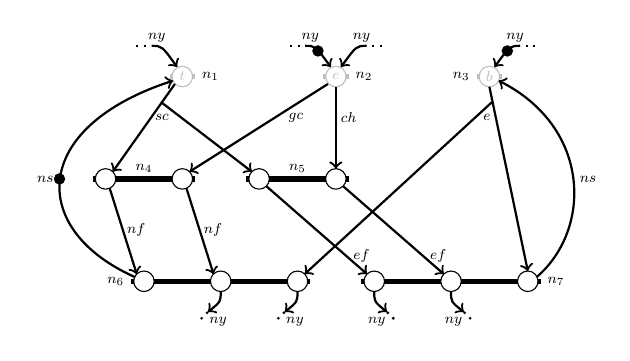
\begin{tikzpicture}[scale=0.65, every node/.style={transform shape}]

\begin{scope}[line width=2pt]
\draw (-1.75,-2) -- (0.25,-2);
\draw (1.25,-2) -- (3.25,-2);
\draw (-1,-4) -- (2.5,-4);
\draw (3.5,-4) -- (7,-4);
\end{scope}

\begin{scope}[line width=2pt, lightgray]
\draw (-0.25,0) -- (0.25,0);
\draw (2.75,0) -- (3.25,0);
\draw (5.75,0) -- (6.25,0);
\end{scope}

\filldraw [lightgray, fill=white]  (0,0)  circle (2mm) node (t0) {\footnotesize $t$};
\filldraw [lightgray, fill=white]  (3,0)  circle (2mm) node (e0) {\footnotesize $e$};
\filldraw [lightgray, fill=white]  (6,0)  circle (2mm) node (b0) {\footnotesize $b$};
\filldraw [fill=white]  (-1.5,-2)  circle (2mm) node (t1) {};
\filldraw [fill=white]  (0,-2)  circle (2mm) node (e1) {};
\filldraw [fill=white]  (1.5,-2)  circle (2mm) node (t2) {};
\filldraw [fill=white]  (3,-2)  circle (2mm) node (e2) {};
\filldraw [fill=white]  (-0.75,-4)  circle (2mm) node (t5) {};
\filldraw [fill=white]  (0.75,-4)  circle (2mm) node (e5) {};
\filldraw [fill=white]  (2.25,-4)  circle (2mm) node (b5) {};
\filldraw [fill=white]  (3.75,-4)  circle (2mm) node (t6) {};
\filldraw [fill=white]  (5.25,-4)  circle (2mm) node (e6) {};
\filldraw [fill=white]  (6.75,-4)  circle (2mm) node (b6) {};

\node at (0.55,0) {\footnotesize $n_1$};
\node at (3.55,0) {\footnotesize$n_2$};
\node at (5.45,0) {\footnotesize $n_3$};
\node at (-0.75,-1.8) {\footnotesize $n_4$};
\node at (2.25,-1.8) {\footnotesize $n_5$};
\node at (-1.3,-4) {\footnotesize $n_6$};
\node at (7.3,-4) {\footnotesize $n_7$};

\node at (-0.4, -0.8) {\footnotesize $sc$};
\node at (2.22, -0.8) {\footnotesize $gc$};
\node at (3.25, -0.8) {\footnotesize $ch$};
\node at (5.95, -0.8) {\footnotesize $e$};
\node at (-0.9,-3) {\footnotesize $nf$};
\node at (0.6, -3) {\footnotesize $nf$};
\node at (3.5,-3.5) {\footnotesize $ef$};
\node at (5,-3.5) {\footnotesize $ef$};
\node at (0.7, -4.8) {\footnotesize $ny$};
\node at (2.2, -4.8) {\footnotesize $ny$};
\node at (3.8, -4.8) {\footnotesize $ny$};
\node at (5.3, -4.8) {\footnotesize $ny$};
\node at (-0.5, 0.75) {\footnotesize $ny$};
\node at (2.5, 0.75) {\footnotesize $ny$};
\node at (3.5, 0.75) {\footnotesize $ny$};
\node at (6.5, 0.75) {\footnotesize $ny$};

\begin{scope}[thick,->]
\draw (-0.145, -0.145) -- (-1.36, -1.86); %t0-t1
\draw (-0.415, -0.5) -- (1.36, -1.86); %t0-t2
\draw (2.845, -0.145) -- (0.14, -1.86); %e0-e1
\draw (3, -0.2) -- (3, -1.8); %e0-e2
\draw (-1.5, -2) + (0.08, -0.18) -- (-0.89, -3.86); %t1-t3
\draw (0, -2) + (0.08, -0.18) -- (0.61, -3.86); %e1-e3
\draw (1.5, -2) + (0.145, -0.145) -- (3.61, -3.86); %t2-t4
\draw (3, -2) + (0.145, -0.145) -- (5.11, -3.86); %e2-e4
\draw (6.05, -0.5) -- (2.39, -3.86); %b0-b3
\draw (6, -0.2) -- (6.75, -3.8); %b0-b4
\draw (-0.92, -3.92) .. controls (-3, -3) and (-3, -1) .. (-0.18, -0.08) node [midway, left] {\footnotesize $ns$}; %t3-t0
\draw (6.92, -3.92) .. controls (8, -3) and (8, -1) .. (6.18, -0.08) node [midway, right] {\footnotesize $ns$}; %b4-b0
\draw (0.75,-4.2) .. controls (0.75, -4.4) .. (0.5,-4.6) ; %e3-e0
\draw (2.25, -4.2) .. controls (2.25, -4.4) .. (2, -4.6); %b3-b0
\draw (3.75, -4.2) .. controls (3.75, -4.4) .. (4, -4.6); %t4-t0
\draw (5.25, -4.2) .. controls (5.25, -4.4) .. (5.5, -4.6); %e4-e0
\draw (-0.6, 0.6) .. controls (-0.4, 0.6) .. (-0.1, 0.185); %t4-t0
\draw (2.4, 0.6) .. controls (2.6, 0.6) .. (2.9, 0.185); %e3-e0
\draw (3.6, 0.6) .. controls (3.4, 0.6) .. (3.1, 0.185); %e4-e0
\draw (6.6, 0.6) .. controls (6.4, 0.6) .. (6.1, 0.185); %b3-b0
\end{scope}

\begin{scope}[thick, dotted]
\draw (-0.9, 0.6) -- (-0.6, 0.6);
\draw (2.1, 0.6) -- (2.4, 0.6);
\draw (3.9, 0.6) -- (3.6, 0.6);
\draw (6.9, 0.6) -- (6.6, 0.6);
\draw (0.5,-4.6) -- (0.3, -4.8);
\draw (2, -4.6) -- (1.8, -4.8);
\draw (4, -4.6) -- (4.2, -4.8);
\draw (5.5, -4.6) -- (5.7, -4.8);
\end{scope}

\filldraw [fill=black]  (-2.4,-2)  circle (1mm);
\filldraw [fill=black]  (2.65,0.5)  circle (1mm);
\filldraw [fill=black]  (6.35,0.5)  circle (1mm);

\end{tikzpicture}
\end{minipage}
\begin{minipage}{.49\textwidth}
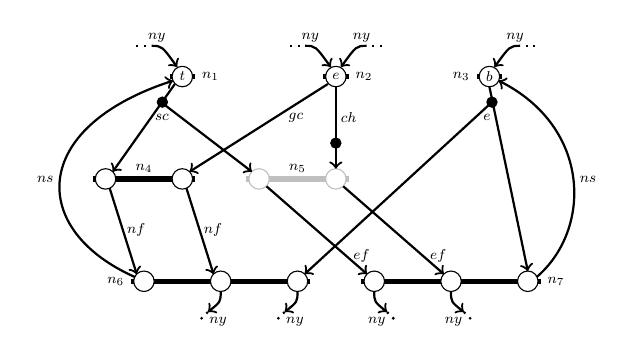
\begin{tikzpicture}[scale=0.65, every node/.style={transform shape}]

\begin{scope}[line width=2pt]
\draw (-0.25,0) -- (0.25,0);
\draw (2.75,0) -- (3.25,0);
\draw (5.75,0) -- (6.25,0);
\draw (-1.75,-2) -- (0.25,-2);
\draw (-1,-4) -- (2.5,-4);
\draw (3.5,-4) -- (7,-4);
\end{scope}

\draw [line width=2pt, lightgray] (1.25,-2) -- (3.25,-2);

\filldraw [fill=white]  (0,0)  circle (2mm) node (t0) {\footnotesize $t$};
\filldraw [fill=white]  (3,0)  circle (2mm) node (e0) {\footnotesize $e$};
\filldraw [fill=white]  (6,0)  circle (2mm) node (b0) {\footnotesize $b$};
\filldraw [fill=white]  (-1.5,-2)  circle (2mm) node (t1) {};
\filldraw [fill=white]  (0,-2)  circle (2mm) node (e1) {};
\filldraw [lightgray, fill=white]  (1.5,-2)  circle (2mm) node (t2) {};
\filldraw [lightgray, fill=white]  (3,-2)  circle (2mm) node (e2) {};
\filldraw [fill=white]  (-0.75,-4)  circle (2mm) node (t5) {};
\filldraw [fill=white]  (0.75,-4)  circle (2mm) node (e5) {};
\filldraw [fill=white]  (2.25,-4)  circle (2mm) node (b5) {};
\filldraw [fill=white]  (3.75,-4)  circle (2mm) node (t6) {};
\filldraw [fill=white]  (5.25,-4)  circle (2mm) node (e6) {};
\filldraw [fill=white]  (6.75,-4)  circle (2mm) node (b6) {};

\node at (0.55,0) {\footnotesize $n_1$};
\node at (3.55,0) {\footnotesize$n_2$};
\node at (5.45,0) {\footnotesize $n_3$};
\node at (-0.75,-1.8) {\footnotesize $n_4$};
\node at (2.25,-1.8) {\footnotesize $n_5$};
\node at (-1.3,-4) {\footnotesize $n_6$};
\node at (7.3,-4) {\footnotesize $n_7$};

\node at (-0.4, -0.8) {\footnotesize $sc$};
\node at (2.22, -0.8) {\footnotesize $gc$};
\node at (3.25, -0.8) {\footnotesize $ch$};
\node at (5.95, -0.8) {\footnotesize $e$};
\node at (-0.9,-3) {\footnotesize $nf$};
\node at (0.6, -3) {\footnotesize $nf$};
\node at (3.5,-3.5) {\footnotesize $ef$};
\node at (5,-3.5) {\footnotesize $ef$};
\node at (0.7, -4.8) {\footnotesize $ny$};
\node at (2.2, -4.8) {\footnotesize $ny$};
\node at (3.8, -4.8) {\footnotesize $ny$};
\node at (5.3, -4.8) {\footnotesize $ny$};
\node at (-0.5, 0.75) {\footnotesize $ny$};
\node at (2.5, 0.75) {\footnotesize $ny$};
\node at (3.5, 0.75) {\footnotesize $ny$};
\node at (6.5, 0.75) {\footnotesize $ny$};

\begin{scope}[thick,->]
\draw (-0.145, -0.145) -- (-1.36, -1.86); %t0-t1
\draw (-0.415, -0.5) -- (1.36, -1.86); %t0-t2
\draw (2.845, -0.145) -- (0.14, -1.86); %e0-e1
\draw (3, -0.2) -- (3, -1.8); %e0-e2
\draw (-1.5, -2) + (0.08, -0.18) -- (-0.89, -3.86); %t1-t3
\draw (0, -2) + (0.08, -0.18) -- (0.61, -3.86); %e1-e3
\draw (1.5, -2) + (0.145, -0.145) -- (3.61, -3.86); %t2-t4
\draw (3, -2) + (0.145, -0.145) -- (5.11, -3.86); %e2-e4
\draw (6.05, -0.5) -- (2.39, -3.86); %b0-b3
\draw (6, -0.2) -- (6.75, -3.8); %b0-b4
\draw (-0.92, -3.92) .. controls (-3, -3) and (-3, -1) .. (-0.18, -0.08) node [midway, left] {\footnotesize $ns$}; %t3-t0
\draw (6.92, -3.92) .. controls (8, -3) and (8, -1) .. (6.18, -0.08) node [midway, right] {\footnotesize $ns$}; %b4-b0
\draw (0.75,-4.2) .. controls (0.75, -4.4) .. (0.5,-4.6) ; %e3-e0
\draw (2.25, -4.2) .. controls (2.25, -4.4) .. (2, -4.6); %b3-b0
\draw (3.75, -4.2) .. controls (3.75, -4.4) .. (4, -4.6); %t4-t0
\draw (5.25, -4.2) .. controls (5.25, -4.4) .. (5.5, -4.6); %e4-e0
\draw (-0.6, 0.6) .. controls (-0.4, 0.6) .. (-0.1, 0.185); %t4-t0
\draw (2.4, 0.6) .. controls (2.6, 0.6) .. (2.9, 0.185); %e3-e0
\draw (3.6, 0.6) .. controls (3.4, 0.6) .. (3.1, 0.185); %e4-e0
\draw (6.6, 0.6) .. controls (6.4, 0.6) .. (6.1, 0.185); %b3-b0
\end{scope}

\begin{scope}[thick, dotted]
\draw (-0.9, 0.6) -- (-0.6, 0.6);
\draw (2.1, 0.6) -- (2.4, 0.6);
\draw (3.9, 0.6) -- (3.6, 0.6);
\draw (6.9, 0.6) -- (6.6, 0.6);
\draw (0.5,-4.6) -- (0.3, -4.8);
\draw (2, -4.6) -- (1.8, -4.8);
\draw (4, -4.6) -- (4.2, -4.8);
\draw (5.5, -4.6) -- (5.7, -4.8);
\end{scope}

\filldraw [fill=black]  (-0.39,-0.5)  circle (1mm);
\filldraw [fill=black]  (3,-1.3)  circle (1mm);
\filldraw [fill=black]  (6.05,-0.5)  circle (1mm);

\end{tikzpicture}
\end{minipage}
\begin{minipage}{.49\textwidth}
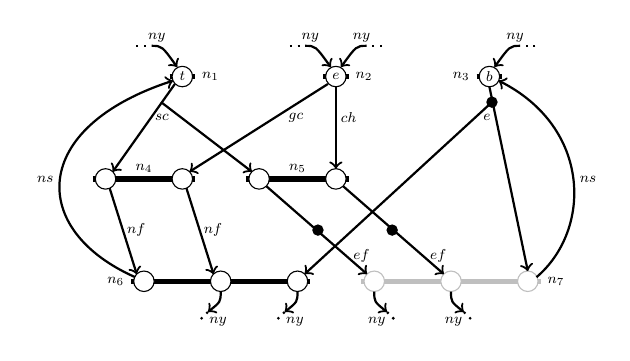
\begin{tikzpicture}[scale=0.65, every node/.style={transform shape}]

\begin{scope}[line width=2pt]
\draw (-0.25,0) -- (0.25,0);
\draw (2.75,0) -- (3.25,0);
\draw (5.75,0) -- (6.25,0);
\draw (-1.75,-2) -- (0.25,-2);
\draw (1.25,-2) -- (3.25,-2);
\draw (-1,-4) -- (2.5,-4);
\end{scope}

\draw [line width=2pt, lightgray] (3.5,-4) -- (7,-4);

\filldraw [fill=white]  (0,0)  circle (2mm) node (t0) {\footnotesize $t$};
\filldraw [fill=white]  (3,0)  circle (2mm) node (e0) {\footnotesize $e$};
\filldraw [fill=white]  (6,0)  circle (2mm) node (b0) {\footnotesize $b$};
\filldraw [fill=white]  (-1.5,-2)  circle (2mm) node (t1) {};
\filldraw [fill=white]  (0,-2)  circle (2mm) node (e1) {};
\filldraw [fill=white]  (1.5,-2)  circle (2mm) node (t2) {};
\filldraw [fill=white]  (3,-2)  circle (2mm) node (e2) {};
\filldraw [fill=white]  (-0.75,-4)  circle (2mm) node (t5) {};
\filldraw [fill=white]  (0.75,-4)  circle (2mm) node (e5) {};
\filldraw [fill=white]  (2.25,-4)  circle (2mm) node (b5) {};
\filldraw [lightgray, fill=white]  (3.75,-4)  circle (2mm) node (t6) {};
\filldraw [lightgray, fill=white]  (5.25,-4)  circle (2mm) node (e6) {};
\filldraw [lightgray, fill=white]  (6.75,-4)  circle (2mm) node (b6) {};

\node at (0.55,0) {\footnotesize $n_1$};
\node at (3.55,0) {\footnotesize$n_2$};
\node at (5.45,0) {\footnotesize $n_3$};
\node at (-0.75,-1.8) {\footnotesize $n_4$};
\node at (2.25,-1.8) {\footnotesize $n_5$};
\node at (-1.3,-4) {\footnotesize $n_6$};
\node at (7.3,-4) {\footnotesize $n_7$};

\node at (-0.4, -0.8) {\footnotesize $sc$};
\node at (2.22, -0.8) {\footnotesize $gc$};
\node at (3.25, -0.8) {\footnotesize $ch$};
\node at (5.95, -0.8) {\footnotesize $e$};
\node at (-0.9,-3) {\footnotesize $nf$};
\node at (0.6, -3) {\footnotesize $nf$};
\node at (3.5,-3.5) {\footnotesize $ef$};
\node at (5,-3.5) {\footnotesize $ef$};
\node at (0.7, -4.8) {\footnotesize $ny$};
\node at (2.2, -4.8) {\footnotesize $ny$};
\node at (3.8, -4.8) {\footnotesize $ny$};
\node at (5.3, -4.8) {\footnotesize $ny$};
\node at (-0.5, 0.75) {\footnotesize $ny$};
\node at (2.5, 0.75) {\footnotesize $ny$};
\node at (3.5, 0.75) {\footnotesize $ny$};
\node at (6.5, 0.75) {\footnotesize $ny$};

\begin{scope}[thick,->]
\draw (-0.145, -0.145) -- (-1.36, -1.86); %t0-t1
\draw (-0.415, -0.5) -- (1.36, -1.86); %t0-t2
\draw (2.845, -0.145) -- (0.14, -1.86); %e0-e1
\draw (3, -0.2) -- (3, -1.8); %e0-e2
\draw (-1.5, -2) + (0.08, -0.18) -- (-0.89, -3.86); %t1-t3
\draw (0, -2) + (0.08, -0.18) -- (0.61, -3.86); %e1-e3
\draw (1.5, -2) + (0.145, -0.145) -- (3.61, -3.86); %t2-t4
\draw (3, -2) + (0.145, -0.145) -- (5.11, -3.86); %e2-e4
\draw (6.05, -0.5) -- (2.39, -3.86); %b0-b3
\draw (6, -0.2) -- (6.75, -3.8); %b0-b4
\draw (-0.92, -3.92) .. controls (-3, -3) and (-3, -1) .. (-0.18, -0.08) node [midway, left] {\footnotesize $ns$}; %t3-t0
\draw (6.92, -3.92) .. controls (8, -3) and (8, -1) .. (6.18, -0.08) node [midway, right] {\footnotesize $ns$}; %b4-b0
\draw (0.75,-4.2) .. controls (0.75, -4.4) .. (0.5,-4.6) ; %e3-e0
\draw (2.25, -4.2) .. controls (2.25, -4.4) .. (2, -4.6); %b3-b0
\draw (3.75, -4.2) .. controls (3.75, -4.4) .. (4, -4.6); %t4-t0
\draw (5.25, -4.2) .. controls (5.25, -4.4) .. (5.5, -4.6); %e4-e0
\draw (-0.6, 0.6) .. controls (-0.4, 0.6) .. (-0.1, 0.185); %t4-t0
\draw (2.4, 0.6) .. controls (2.6, 0.6) .. (2.9, 0.185); %e3-e0
\draw (3.6, 0.6) .. controls (3.4, 0.6) .. (3.1, 0.185); %e4-e0
\draw (6.6, 0.6) .. controls (6.4, 0.6) .. (6.1, 0.185); %b3-b0
\end{scope}

\begin{scope}[thick, dotted]
\draw (-0.9, 0.6) -- (-0.6, 0.6);
\draw (2.1, 0.6) -- (2.4, 0.6);
\draw (3.9, 0.6) -- (3.6, 0.6);
\draw (6.9, 0.6) -- (6.6, 0.6);
\draw (0.5,-4.6) -- (0.3, -4.8);
\draw (2, -4.6) -- (1.8, -4.8);
\draw (4, -4.6) -- (4.2, -4.8);
\draw (5.5, -4.6) -- (5.7, -4.8);
\end{scope}

\filldraw [fill=black]  (2.65,-3)  circle (1mm);
\filldraw [fill=black]  (4.1,-3)  circle (1mm);
\filldraw [fill=black]  (6.05,-0.5)  circle (1mm);

\end{tikzpicture}
\end{minipage}
\begin{minipage}{.49\textwidth}
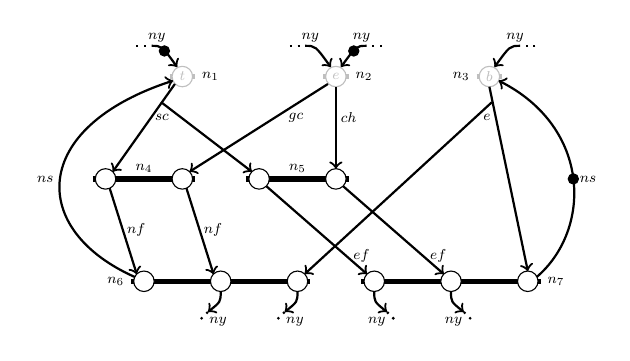
\begin{tikzpicture}[scale=0.65, every node/.style={transform shape}]

\begin{scope}[line width=2pt]
\draw (-1.75,-2) -- (0.25,-2);
\draw (1.25,-2) -- (3.25,-2);
\draw (-1,-4) -- (2.5,-4);
\draw (3.5,-4) -- (7,-4);
\end{scope}

\begin{scope}[line width=2pt, lightgray]
\draw (-0.25,0) -- (0.25,0);
\draw (2.75,0) -- (3.25,0);
\draw (5.75,0) -- (6.25,0);
\end{scope}

\filldraw [lightgray, fill=white]  (0,0)  circle (2mm) node (t0) {\footnotesize $t$};
\filldraw [lightgray, fill=white]  (3,0)  circle (2mm) node (e0) {\footnotesize $e$};
\filldraw [lightgray, fill=white]  (6,0)  circle (2mm) node (b0) {\footnotesize $b$};
\filldraw [fill=white]  (-1.5,-2)  circle (2mm) node (t1) {};
\filldraw [fill=white]  (0,-2)  circle (2mm) node (e1) {};
\filldraw [fill=white]  (1.5,-2)  circle (2mm) node (t2) {};
\filldraw [fill=white]  (3,-2)  circle (2mm) node (e2) {};
\filldraw [fill=white]  (-0.75,-4)  circle (2mm) node (t5) {};
\filldraw [fill=white]  (0.75,-4)  circle (2mm) node (e5) {};
\filldraw [fill=white]  (2.25,-4)  circle (2mm) node (b5) {};
\filldraw [fill=white]  (3.75,-4)  circle (2mm) node (t6) {};
\filldraw [fill=white]  (5.25,-4)  circle (2mm) node (e6) {};
\filldraw [fill=white]  (6.75,-4)  circle (2mm) node (b6) {};

\node at (0.55,0) {\footnotesize $n_1$};
\node at (3.55,0) {\footnotesize$n_2$};
\node at (5.45,0) {\footnotesize $n_3$};
\node at (-0.75,-1.8) {\footnotesize $n_4$};
\node at (2.25,-1.8) {\footnotesize $n_5$};
\node at (-1.3,-4) {\footnotesize $n_6$};
\node at (7.3,-4) {\footnotesize $n_7$};

\node at (-0.4, -0.8) {\footnotesize $sc$};
\node at (2.22, -0.8) {\footnotesize $gc$};
\node at (3.25, -0.8) {\footnotesize $ch$};
\node at (5.95, -0.8) {\footnotesize $e$};
\node at (-0.9,-3) {\footnotesize $nf$};
\node at (0.6, -3) {\footnotesize $nf$};
\node at (3.5,-3.5) {\footnotesize $ef$};
\node at (5,-3.5) {\footnotesize $ef$};
\node at (0.7, -4.8) {\footnotesize $ny$};
\node at (2.2, -4.8) {\footnotesize $ny$};
\node at (3.8, -4.8) {\footnotesize $ny$};
\node at (5.3, -4.8) {\footnotesize $ny$};
\node at (-0.5, 0.75) {\footnotesize $ny$};
\node at (2.5, 0.75) {\footnotesize $ny$};
\node at (3.5, 0.75) {\footnotesize $ny$};
\node at (6.5, 0.75) {\footnotesize $ny$};

\begin{scope}[thick,->]
\draw (-0.145, -0.145) -- (-1.36, -1.86); %t0-t1
\draw (-0.415, -0.5) -- (1.36, -1.86); %t0-t2
\draw (2.845, -0.145) -- (0.14, -1.86); %e0-e1
\draw (3, -0.2) -- (3, -1.8); %e0-e2
\draw (-1.5, -2) + (0.08, -0.18) -- (-0.89, -3.86); %t1-t3
\draw (0, -2) + (0.08, -0.18) -- (0.61, -3.86); %e1-e3
\draw (1.5, -2) + (0.145, -0.145) -- (3.61, -3.86); %t2-t4
\draw (3, -2) + (0.145, -0.145) -- (5.11, -3.86); %e2-e4
\draw (6.05, -0.5) -- (2.39, -3.86); %b0-b3
\draw (6, -0.2) -- (6.75, -3.8); %b0-b4
\draw (-0.92, -3.92) .. controls (-3, -3) and (-3, -1) .. (-0.18, -0.08) node [midway, left] {\footnotesize $ns$}; %t3-t0
\draw (6.92, -3.92) .. controls (8, -3) and (8, -1) .. (6.18, -0.08) node [midway, right] {\footnotesize $ns$}; %b4-b0
\draw (0.75,-4.2) .. controls (0.75, -4.4) .. (0.5,-4.6) ; %e3-e0
\draw (2.25, -4.2) .. controls (2.25, -4.4) .. (2, -4.6); %b3-b0
\draw (3.75, -4.2) .. controls (3.75, -4.4) .. (4, -4.6); %t4-t0
\draw (5.25, -4.2) .. controls (5.25, -4.4) .. (5.5, -4.6); %e4-e0
\draw (-0.6, 0.6) .. controls (-0.4, 0.6) .. (-0.1, 0.185); %t4-t0
\draw (2.4, 0.6) .. controls (2.6, 0.6) .. (2.9, 0.185); %e3-e0
\draw (3.6, 0.6) .. controls (3.4, 0.6) .. (3.1, 0.185); %e4-e0
\draw (6.6, 0.6) .. controls (6.4, 0.6) .. (6.1, 0.185); %b3-b0
\end{scope}

\begin{scope}[thick, dotted]
\draw (-0.9, 0.6) -- (-0.6, 0.6);
\draw (2.1, 0.6) -- (2.4, 0.6);
\draw (3.9, 0.6) -- (3.6, 0.6);
\draw (6.9, 0.6) -- (6.6, 0.6);
\draw (0.5,-4.6) -- (0.3, -4.8);
\draw (2, -4.6) -- (1.8, -4.8);
\draw (4, -4.6) -- (4.2, -4.8);
\draw (5.5, -4.6) -- (5.7, -4.8);
\end{scope}

\filldraw [fill=black]  (-0.35,0.5)  circle (1mm);
\filldraw [fill=black]  (3.35,0.5)  circle (1mm);
\filldraw [fill=black]  (7.64,-2)  circle (1mm);

\end{tikzpicture}
\end{minipage}
\begin{minipage}{.49\textwidth}
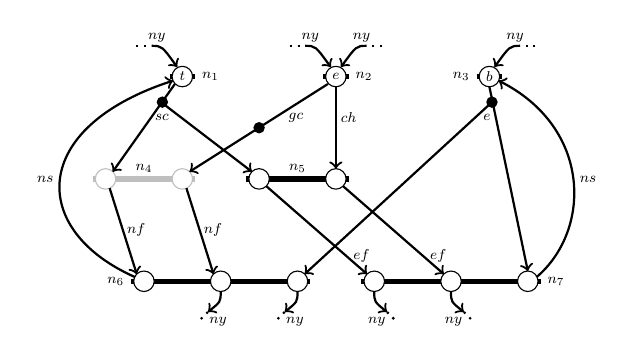
\begin{tikzpicture}[scale=0.65, every node/.style={transform shape}]

\begin{scope}[line width=2pt]
\draw (-0.25,0) -- (0.25,0);
\draw (2.75,0) -- (3.25,0);
\draw (5.75,0) -- (6.25,0);
\draw (1.25,-2) -- (3.25,-2);
\draw (-1,-4) -- (2.5,-4);
\draw (3.5,-4) -- (7,-4);
\end{scope}

\draw [line width=2pt, lightgray] (-1.75,-2) -- (0.25,-2);

\filldraw [fill=white]  (0,0)  circle (2mm) node (t0) {\footnotesize $t$};
\filldraw [fill=white]  (3,0)  circle (2mm) node (e0) {\footnotesize $e$};
\filldraw [fill=white]  (6,0)  circle (2mm) node (b0) {\footnotesize $b$};
\filldraw [lightgray, fill=white]  (-1.5,-2)  circle (2mm) node (t1) {};
\filldraw [lightgray, fill=white]  (0,-2)  circle (2mm) node (e1) {};
\filldraw [fill=white]  (1.5,-2)  circle (2mm) node (t2) {};
\filldraw [fill=white]  (3,-2)  circle (2mm) node (e2) {};
\filldraw [fill=white]  (-0.75,-4)  circle (2mm) node (t5) {};
\filldraw [fill=white]  (0.75,-4)  circle (2mm) node (e5) {};
\filldraw [fill=white]  (2.25,-4)  circle (2mm) node (b5) {};
\filldraw [fill=white]  (3.75,-4)  circle (2mm) node (t6) {};
\filldraw [fill=white]  (5.25,-4)  circle (2mm) node (e6) {};
\filldraw [fill=white]  (6.75,-4)  circle (2mm) node (b6) {};

\node at (0.55,0) {\footnotesize $n_1$};
\node at (3.55,0) {\footnotesize$n_2$};
\node at (5.45,0) {\footnotesize $n_3$};
\node at (-0.75,-1.8) {\footnotesize $n_4$};
\node at (2.25,-1.8) {\footnotesize $n_5$};
\node at (-1.3,-4) {\footnotesize $n_6$};
\node at (7.3,-4) {\footnotesize $n_7$};

\node at (-0.4, -0.8) {\footnotesize $sc$};
\node at (2.22, -0.8) {\footnotesize $gc$};
\node at (3.25, -0.8) {\footnotesize $ch$};
\node at (5.95, -0.8) {\footnotesize $e$};
\node at (-0.9,-3) {\footnotesize $nf$};
\node at (0.6, -3) {\footnotesize $nf$};
\node at (3.5,-3.5) {\footnotesize $ef$};
\node at (5,-3.5) {\footnotesize $ef$};
\node at (0.7, -4.8) {\footnotesize $ny$};
\node at (2.2, -4.8) {\footnotesize $ny$};
\node at (3.8, -4.8) {\footnotesize $ny$};
\node at (5.3, -4.8) {\footnotesize $ny$};
\node at (-0.5, 0.75) {\footnotesize $ny$};
\node at (2.5, 0.75) {\footnotesize $ny$};
\node at (3.5, 0.75) {\footnotesize $ny$};
\node at (6.5, 0.75) {\footnotesize $ny$};

\begin{scope}[thick,->]
\draw (-0.145, -0.145) -- (-1.36, -1.86); %t0-t1
\draw (-0.415, -0.5) -- (1.36, -1.86); %t0-t2
\draw (2.845, -0.145) -- (0.14, -1.86); %e0-e1
\draw (3, -0.2) -- (3, -1.8); %e0-e2
\draw (-1.5, -2) + (0.08, -0.18) -- (-0.89, -3.86); %t1-t3
\draw (0, -2) + (0.08, -0.18) -- (0.61, -3.86); %e1-e3
\draw (1.5, -2) + (0.145, -0.145) -- (3.61, -3.86); %t2-t4
\draw (3, -2) + (0.145, -0.145) -- (5.11, -3.86); %e2-e4
\draw (6.05, -0.5) -- (2.39, -3.86); %b0-b3
\draw (6, -0.2) -- (6.75, -3.8); %b0-b4
\draw (-0.92, -3.92) .. controls (-3, -3) and (-3, -1) .. (-0.18, -0.08) node [midway, left] {\footnotesize $ns$}; %t3-t0
\draw (6.92, -3.92) .. controls (8, -3) and (8, -1) .. (6.18, -0.08) node [midway, right] {\footnotesize $ns$}; %b4-b0
\draw (0.75,-4.2) .. controls (0.75, -4.4) .. (0.5,-4.6) ; %e3-e0
\draw (2.25, -4.2) .. controls (2.25, -4.4) .. (2, -4.6); %b3-b0
\draw (3.75, -4.2) .. controls (3.75, -4.4) .. (4, -4.6); %t4-t0
\draw (5.25, -4.2) .. controls (5.25, -4.4) .. (5.5, -4.6); %e4-e0
\draw (-0.6, 0.6) .. controls (-0.4, 0.6) .. (-0.1, 0.185); %t4-t0
\draw (2.4, 0.6) .. controls (2.6, 0.6) .. (2.9, 0.185); %e3-e0
\draw (3.6, 0.6) .. controls (3.4, 0.6) .. (3.1, 0.185); %e4-e0
\draw (6.6, 0.6) .. controls (6.4, 0.6) .. (6.1, 0.185); %b3-b0
\end{scope}

\begin{scope}[thick, dotted]
\draw (-0.9, 0.6) -- (-0.6, 0.6);
\draw (2.1, 0.6) -- (2.4, 0.6);
\draw (3.9, 0.6) -- (3.6, 0.6);
\draw (6.9, 0.6) -- (6.6, 0.6);
\draw (0.5,-4.6) -- (0.3, -4.8);
\draw (2, -4.6) -- (1.8, -4.8);
\draw (4, -4.6) -- (4.2, -4.8);
\draw (5.5, -4.6) -- (5.7, -4.8);
\end{scope}

\filldraw [fill=black]  (-0.39,-0.5)  circle (1mm);
\filldraw [fill=black]  (1.5,-1)  circle (1mm);
\filldraw [fill=black]  (6.05,-0.5)  circle (1mm);

\end{tikzpicture}
\end{minipage}
\begin{minipage}{.49\textwidth}
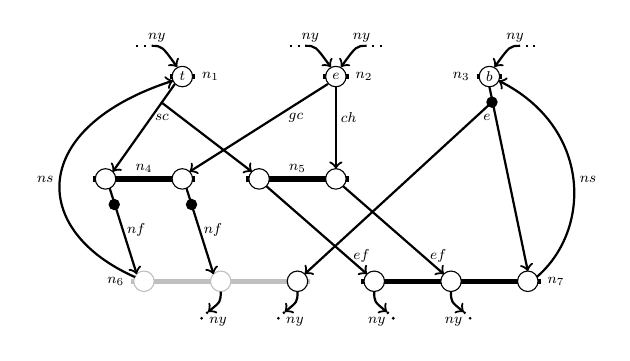
\begin{tikzpicture}[scale=0.65, every node/.style={transform shape}]

\begin{scope}[line width=2pt]
\draw (-0.25,0) -- (0.25,0);
\draw (2.75,0) -- (3.25,0);
\draw (5.75,0) -- (6.25,0);
\draw (-1.75,-2) -- (0.25,-2);
\draw (1.25,-2) -- (3.25,-2);
\draw (3.5,-4) -- (7,-4);
\end{scope}

\draw [line width=2pt, lightgray] (-1,-4) -- (2.5,-4);

\filldraw [fill=white]  (0,0)  circle (2mm) node (t0) {\footnotesize $t$};
\filldraw [fill=white]  (3,0)  circle (2mm) node (e0) {\footnotesize $e$};
\filldraw [fill=white]  (6,0)  circle (2mm) node (b0) {\footnotesize $b$};
\filldraw [fill=white]  (-1.5,-2)  circle (2mm) node (t1) {};
\filldraw [fill=white]  (0,-2)  circle (2mm) node (e1) {};
\filldraw [fill=white]  (1.5,-2)  circle (2mm) node (t2) {};
\filldraw [fill=white]  (3,-2)  circle (2mm) node (e2) {};
\filldraw [lightgray, fill=white]  (-0.75,-4)  circle (2mm) node (t5) {};
\filldraw [lightgray, fill=white]  (0.75,-4)  circle (2mm) node (e5) {};
\filldraw [fill=white]  (2.25,-4)  circle (2mm) node (b5) {};
\filldraw [fill=white]  (3.75,-4)  circle (2mm) node (t6) {};
\filldraw [fill=white]  (5.25,-4)  circle (2mm) node (e6) {};
\filldraw [fill=white]  (6.75,-4)  circle (2mm) node (b6) {};

\node at (0.55,0) {\footnotesize $n_1$};
\node at (3.55,0) {\footnotesize$n_2$};
\node at (5.45,0) {\footnotesize $n_3$};
\node at (-0.75,-1.8) {\footnotesize $n_4$};
\node at (2.25,-1.8) {\footnotesize $n_5$};
\node at (-1.3,-4) {\footnotesize $n_6$};
\node at (7.3,-4) {\footnotesize $n_7$};

\node at (-0.4, -0.8) {\footnotesize $sc$};
\node at (2.22, -0.8) {\footnotesize $gc$};
\node at (3.25, -0.8) {\footnotesize $ch$};
\node at (5.95, -0.8) {\footnotesize $e$};
\node at (-0.9,-3) {\footnotesize $nf$};
\node at (0.6, -3) {\footnotesize $nf$};
\node at (3.5,-3.5) {\footnotesize $ef$};
\node at (5,-3.5) {\footnotesize $ef$};
\node at (0.7, -4.8) {\footnotesize $ny$};
\node at (2.2, -4.8) {\footnotesize $ny$};
\node at (3.8, -4.8) {\footnotesize $ny$};
\node at (5.3, -4.8) {\footnotesize $ny$};
\node at (-0.5, 0.75) {\footnotesize $ny$};
\node at (2.5, 0.75) {\footnotesize $ny$};
\node at (3.5, 0.75) {\footnotesize $ny$};
\node at (6.5, 0.75) {\footnotesize $ny$};

\begin{scope}[thick,->]
\draw (-0.145, -0.145) -- (-1.36, -1.86); %t0-t1
\draw (-0.415, -0.5) -- (1.36, -1.86); %t0-t2
\draw (2.845, -0.145) -- (0.14, -1.86); %e0-e1
\draw (3, -0.2) -- (3, -1.8); %e0-e2
\draw (-1.5, -2) + (0.08, -0.18) -- (-0.89, -3.86); %t1-t3
\draw (0, -2) + (0.08, -0.18) -- (0.61, -3.86); %e1-e3
\draw (1.5, -2) + (0.145, -0.145) -- (3.61, -3.86); %t2-t4
\draw (3, -2) + (0.145, -0.145) -- (5.11, -3.86); %e2-e4
\draw (6.05, -0.5) -- (2.39, -3.86); %b0-b3
\draw (6, -0.2) -- (6.75, -3.8); %b0-b4
\draw (-0.92, -3.92) .. controls (-3, -3) and (-3, -1) .. (-0.18, -0.08) node [midway, left] {\footnotesize $ns$}; %t3-t0
\draw (6.92, -3.92) .. controls (8, -3) and (8, -1) .. (6.18, -0.08) node [midway, right] {\footnotesize $ns$}; %b4-b0
\draw (0.75,-4.2) .. controls (0.75, -4.4) .. (0.5,-4.6) ; %e3-e0
\draw (2.25, -4.2) .. controls (2.25, -4.4) .. (2, -4.6); %b3-b0
\draw (3.75, -4.2) .. controls (3.75, -4.4) .. (4, -4.6); %t4-t0
\draw (5.25, -4.2) .. controls (5.25, -4.4) .. (5.5, -4.6); %e4-e0
\draw (-0.6, 0.6) .. controls (-0.4, 0.6) .. (-0.1, 0.185); %t4-t0
\draw (2.4, 0.6) .. controls (2.6, 0.6) .. (2.9, 0.185); %e3-e0
\draw (3.6, 0.6) .. controls (3.4, 0.6) .. (3.1, 0.185); %e4-e0
\draw (6.6, 0.6) .. controls (6.4, 0.6) .. (6.1, 0.185); %b3-b0
\end{scope}

\begin{scope}[thick, dotted]
\draw (-0.9, 0.6) -- (-0.6, 0.6);
\draw (2.1, 0.6) -- (2.4, 0.6);
\draw (3.9, 0.6) -- (3.6, 0.6);
\draw (6.9, 0.6) -- (6.6, 0.6);
\draw (0.5,-4.6) -- (0.3, -4.8);
\draw (2, -4.6) -- (1.8, -4.8);
\draw (4, -4.6) -- (4.2, -4.8);
\draw (5.5, -4.6) -- (5.7, -4.8);
\end{scope}

\filldraw [fill=black]  (-1.33,-2.5)  circle (1mm);
\filldraw [fill=black]  (0.18,-2.5)  circle (1mm);
\filldraw [fill=black]  (6.05,-0.5)  circle (1mm);

\end{tikzpicture}
\end{minipage}
\caption{This is a possible run of the partial distributed negotiations shown in Figure ~\ref{fig:pollination}. The  markings are graphically represented by placing tokens (black dots) on the forking points of the hyperarcs (or, if the hyperarc consists of just one arc, then on the arc). The gray nodes denotes the nodes which are enabled by the current marking. Initially $n_1$, $n_2$, and $n_3$ are enabled. After firing $(n_1, sc)$, $(n_2, ch)$, and $(n_3, e)$, the process $t$ is ready to engage in $n_4$ and $n_5$, the process $e$ is ready to engage only in $n_5$, and the process $b$ is ready to engage in $n_6$ and $n_7$. Hence, the only enabled node is $n_5$, and next $(n_5, ef)$ is fired. Few more steps of the run is shown in the above diagram.}
	\label{fig:run}
\end{figure}

This model is sometimes more intuitive than other existing models such as Petri nets, network of automata over distributed alphabet, process algebra etc. This formalism has a graphical representation similar to Petri nets as shown in Figure ~\ref{fig:pollination}. Atomic negotiations are represented as nodes, with a specific representation of the participating agents. For each atomic negotiations (also called \textit{nodes}) we draw a black bar; for each process participating in an atomic negotiation we draw a white circle on the bar, called a \textit{port}. In the example of Figure ~\ref{fig:pollination}, $n_4$ is a node with two processes $t$ and $e$ (drawn as ports in the figure) participating in it. We say that the domain of $n_4$ is $\{t, e\}$. The node $n_3$ has only one process $b$ in its domain. Each node has outgoing actions and all processes in the domain of that node must participate in those actions together. $n_6$ has only one outgoing action $nl$, whereas $n_2$ has two outgoing actions $gc$ and $ch$. Note that the outgoing edges on $sc$ and $e$ are non-deterministic, which is denoted by hyperarcs in the diagram. If the action $sc$ is taken from $n_1$, then the process $t$ is ready to engage in both the nodes $n_4$ and $n_5$. Non-hyperarcs denotes deterministic edges.

The current next possible atomic negotiations are represented as \textit{markings} of negotiations, which denotes the set of nodes that an agent is currently ready to engage in next. Reachable markings are graphically represented by placing tokens (black dots) on the forking points of the hyperarcs (or, if the hyperarc consists of just one arc, then on the arc). A marking $x$ \textit{enables} a node $n$ if all processes in the domain of $n$ is currently ready to engage in $n$. If $x$ enables $n$, then $n$ can take place and its parties agree on an outgoing action $r$; we say that the outcome $(n, r)$ \textit{occurs}. The occurrence of $(n, r)$ produces a next marking $x'$. We write $x \xra{(n, r)} x'$ to denote this, and call it a \textit{small step}. A \textit{run} of a negotiation is a sequence of small steps $x_1 \xra{(n_1, r_1)} x_2 \xra{(n_2, r_2)} \cdots$. A run can be infinite also. We call $\sigma = (n_1, r_1) (n_1, r_1) \dots$ an \textit{occurrence sequence}. A marking $x_k$ is reachable from $x_1$, if $x_1 \xra{\sigma} x_k$. The final node of a negotiation has only one outgoing action, but it does not enable any atom, and hence not shown in diagrams. A marking that does not enable any atom is a \textit{deadlock}. A marking which is reachable from itself but from which the final marking is not reachable is a \textit{livelock}. Figure ~\ref{} shows a run of the partial negotiation of Figure ~\ref{fig:pollination}.

An occurrence sequence of a negotiation can be arbitrarily long, e.g., the occurrence sequence shown in Figure ~\ref{fig:run} can go on forever. Therefore, the set of possible occurrence sequences can be infinite. Since we have markings and steps, an obvious way to describe behaviour with finite means is by \textit{reachability graphs}. The reachability graph of a negotiation has all markings reachable from the initial marking $x_0$ as vertices, and an arc leading from $x$ to $x'$ and annotated by $(n, r)$ whenever $x \xra{(n,r)} x'$. The initial marking $x_0$ is the distinguished initial vertex. Part of a reachability graph of the incomplete distributed negotiations example of Figure ~\ref{fig:pollination} is shown in Figure ~\ref{}.

For a negotiation with more than one proper hyperarc, each occurrence sequence can involve a particular branching of a hyperarc (moreover, an atom can occur more than once, leading to different branches of the same hyperarc). For $k$ hyperarcs with $n$-ary branching, this results in $n^k$ possible patterns. So, the size of the marking graph is exponential in the number of atoms, and the algorithm to decide reachability by computing the reachability graph is single exponential in the number of atoms. It turns out that this cannot be easily avoided, because the problem is PSPACE-complete, and co-NP-hard and in DP for acyclic negotiations. %see later results and include them here

\begin{figure}[t]
\centering
\begin{tikzpicture}[scale=0.6, every node/.style={transform shape}]

\node at (0,0) {$\{\{n_1\}, \{n_2\}, \{n_3\}\}$};
\node at (-6,-3) {$\{\{n_4, n_5\}, \{n_2\}, \{n_3\}\}$};
\node at (-2,-3) {$\{\{n_1\}, \{n_4\}, \{n_3\}\}$};
\node at (2,-3) {$\{\{n_1\}, \{n_5\}, \{n_3\}\}$};
\node at (6,-3) {$\{\{n_1\}, \{n_2\}, \{n_6, n_7\}\}$};
\node at (-10,-6) {$\{\{n_4, n_5\}, \{n_4\}, \{n_3\}\}$};
\node at (-5,-6) {$\{\{n_4, n_5\}, \{n_5\}, \{n_3\}\}$};
\node at (0,-6) {$\{\{n_4, n_5\}, \{n_2\}, \{n_6, n_7\}\}$};
\node at (5,-6) {$\{\{n_1\}, \{n_4\}, \{n_6, n_7\}\}$};
\node at (10,-6) {$\{\{n_1\}, \{n_5\}, \{n_6, n_7\}\}$};
\node at (-9,-9) {$\{\{n_6\}, \{n_6\}, \{n_3\}\}$};
\node at (3,-9) {$\{\{n_4, n_5\}, \{n_4\}, \{n_6, n_7\}\}$};
\node at (-3,-9) {$\{\{n_7\}, \{n_7\}, \{n_3\}\}$};
\node at (9,-9) {$\{\{n_4, n_5\}, \{n_5\}, \{n_6, n_7\}\}$};
\node at (-6,-12) {$\{\{n_6\}, \{n_6\}, \{n_6, n_7\}\}$};
\node at (6,-12) {$\{\{n_7\}, \{n_7\}, \{n_6, n_7\}\}$};

\begin{scope}[-Stealth]
\draw (0,-0.3) -- (-6,-2.7) node [midway, left, above] {\footnotesize $(n_1, sc)$};
\draw (0,-0.3) -- (-2,-2.7) node [midway, left] {\footnotesize $(n_2, gc)$};
\draw (0,-0.3) -- (2,-2.7) node [midway, left] {\footnotesize $(n_2, ch)$};
\draw (0,-0.3) -- (6,-2.7) node [midway, right, above] {\footnotesize $(n_3, e)$};
\draw (-6,-3.3) -- (-10,-5.7) node [midway, left] {\footnotesize $(n_2, gc)$};
\draw (-6,-3.3) -- (-5,-5.7) node [midway, left, above] {\footnotesize $(n_2, ch)$};%
\draw (-6,-3.3) -- (-0.25,-5.7) node [midway, left] {\footnotesize $(n_3, e)$};
\draw (-2,-3.3) -- (-9.5,-5.7) node [midway, left, below] {\footnotesize $(n_1, sc)$};%
\draw (-2,-3.3) -- (4.75,-5.7) node [midway, left] {\footnotesize $(n_3, e)$};
\draw (2,-3.3) -- (-4.5,-5.7) node [midway, left, below] {\footnotesize $(n_1, sc)$};%
\draw (2,-3.3) -- (9.5,-5.7) node [midway, left] {\footnotesize $(n_3, e)$};
\draw (6,-3.3) -- (0.25,-5.7) node [midway, left] {\footnotesize $(n_1, sc)$};
\draw (6,-3.3) -- (5.25,-5.7) node [midway, left, above] {\footnotesize $(n_2, gc)$};%
\draw (6,-3.3) -- (10,-5.7) node [midway, left] {\footnotesize $(n_2, ch)$};
\draw (-10,-6.3) -- (-9,-8.7) node [midway, left] {\footnotesize $(n_4, nf)$};
\draw (-10,-6.3) -- (2.5,-8.7) node [midway, left] {\footnotesize $(n_3, e)$};
\draw (-5,-6.3) -- (-3,-8.7) node [midway, left] {\footnotesize $(n_4, nf)$};
\draw (-5,-6.3) -- (8.5,-8.7) node [midway, left] {\footnotesize $(n_3, e)$};
\draw (0,-6.3) -- (2.75,-8.7) node [midway, left] {\footnotesize $(n_4, nf)$};
\draw (0,-6.3) -- (8.75,-8.7) node [midway, left] {\footnotesize $(n_3, e)$};
\draw (5,-6.3) -- (3,-8.7) node [midway, left] {\footnotesize $(n_4, nf)$};
\draw (10,-6.3) -- (9,-8.7) node [midway, left] {\footnotesize $(n_4, nf)$};
\draw (-9,-9.3) -- (-6,-11.7) node [midway, left] {\footnotesize $(n_4, nf)$};
\draw (-3,-9.3) -- (5.5,-11.7) node [midway, left] {\footnotesize $(n_4, nf)$};
\draw (3,-9.3) -- (-5.5,-11.7) node [midway, left] {\footnotesize $(n_4, nf)$};
\draw (9,-9.3) -- (6,-11.7) node [midway, left] {\footnotesize $(n_4, nf)$};
\draw (-8, -12) .. controls (-15, -9) and (-15, -1) .. (-2, 0);
\draw (8, -12) .. controls (15, -9) and (15, -1) .. (2, 0);
\end{scope}

\end{tikzpicture}
\caption{Reachability graph of the partial example of Figure ~\ref{fig:pollination} \textcolor{teal}{(explain the exponential blow-up here)}}
	\label{fig:rg-pol}
\end{figure}

The negotiation model has been studied and applied to analyzing industrial business processes, typically represented as workflow Petri nets \cite{}. These nets serve as a formal foundation for popular graphical notations such as Business Process Model and Notation (BPMN), EPC, and UML Activity Diagrams \cite{}. Notably, deterministic negotiations are strongly linked to free-choice workflow nets \cite{}, which possess sufficient expressiveness for many business processes, as evidenced by a study showing 70\% of nearly 2000 industrial models are free-choice.
%_____________________________________________________________________________

\section{Contribution}

In our work, we consider the local time semantics for negotiations from \cite{}, where we introduce a real-time aspect to negotiations. In our model of local-timed negotiations, agents have local reference times that evolve independently. Inspired by the model of networks of timed automata, each agent is equipped with a set of local clocks. Similar to timed automata, the outcomes of a negotiation contain guards and resets over the local clocks. As a new feature, we allow some interactions to force the reference clocks of the participating agents to synchronize. This synchronization constraint allows us to model interesting scenarios. Surprisingly, it also gives unlimited computing power. We show that reachability is undecidable for local-timed negotiations with a mixture of synchronized and unsynchronized interactions. 

As a natural question, we move on study different restrictions on the use of synchronized interactions that make the problem decidable. We show that when the negotiation has no interactions that synchronize local times, or when all interactions force a synchronization of local times, reachability is PSPACE-complete. In the general case when, there is a mix of synchronized and unsynchronized interactions, reachability is undecidable.

In the next part of the thesis, we consider a bounded-drift property for an LTN, similar to the notion considered in \cite{} for networks of timed automata. An LTN is said to have drift bounded by $K$ if in every behaviour, the local-time delays can be tightened so that the drift between the local-times of every pair of processes is always bounded by a constant $K$. Similar to \cite{}, we conclude that reachability is decidable for bounded-drift negotiations, by building a region automaton for the set of untimed behaviours. Subsequently, we consider a syntactic fragment of LTNs, called connectedly-communicating negotiations. An LTN is said to be connectedly-communicating, if in every cycle of a behaviour, each agent has a time-synchronizing negotiation with every other agent, either directly or indirectly. This idea is formalized by looking at the so-called marking graph of the underlying untimed negotiation, and by enforcing that a certain communication graph of each loop to be connected. The inspiration for this definition comes from the work of \cite{} on hierarchical message sequence graphs, where a similar idea makes the emptiness problem decidable. The terminology “connectedly-communicating” comes from the work of \cite{} on the distributed controller synthesis problem, which is undecidable in general. Once again the connectedness restriction makes the problem decidable. The setting of \cite{} is slightly different and weaker than our definition: in their fragment, if process $p$ does not hear from $q$ either directly or indirectly, they never participate in a synchronizing action in the future. Towards the end of this manuscript, we comment on how our techniques can be extended to this weaker setting as well.

%_____________________________________________________________________________

\section{Organization of the Thesis}

The thesis is divided into two parts. In the first part of the thesis, Chapter ~\ref{} talks about formalizing negotiations, timed automata, and network of timed automata with some illustrative examples. In Chapter ~\ref{} we study the local-timed negotiations formally and also show that the reachability problem for this model is undecidable. The second part of the thesis talks about various subclasses of LTN for which reachability problem is decidable. Each of these chapters ends with a section on concluding remarks, where a comprehensive summary of the chapter is provided with references to important definitions and results.

%_____________________________________________________________________________

\section{Related works}

A local-time semantics was proposed in the context of networks of timed automata in [4]. Recently, the semantics has been applied to the zone-based verification of reachability [13,14] and B¨uchi reachability properties [16]. Local-time semantics in timed automata has been investigated as a basis for applying partial-order methods. In our current work, we consider local-time semantics as the starting point and make synchronization an option that can be specified explicitly. This allows more independence between the agents and keeps the concurrency between actions of disjoint sets of agents. 

Models mixing concurrency and timing have been widely studied: time Petri nets [18], timed-arc Petri nets [15], time-constrained message sequence charts [2] to name a few. Each model offers a different view of the computation. To our knowledge, a notion of a real-time has not yet been considered for negotiations. With similar motivations as local-time semantics, a notion of a partial-order semantics has been studied for networks of timed automata [17] as well as time Petri nets [7,8]. This semantics can be used to compute finite unfoldings which preserve the concurrency and reachability information concisely [6,5].

Local-timed negotiations were introduced in [10]. It was shown that reachability is decidable in two cases: either when all nodes are timesynchronizing (called the fully synchronizing fragment), or none of the nodes is time-synchronizing (called the synchronization-free fragment). The idea of drifting the bound between processes in a network of timed automata has been studied for networks of timed automata in [7,8]. For networks of timed automata, local-time semantics has been studied in the context of efficient zone-based verification methods. Due to independence, the zone graph computed using the local-time semantics contains diamonds, and hence avoids one dimension of exponential blowup caused due to interleaving of independent actions. In this context, bounded-drift is helpful in coming up with simulation techniques to make the zone graph exploration finite. Related works from the concurrency literature have been mentioned above.

%_____________________________________________________________________________

% About concurrent systems and formal study of concurrency theory
%In the world we live in, concurrency is ubiquitous. For example, the human body is a massively concurrent system, comprising a huge number of cells, all simultaneously evolving and independently engaging in their individual biological processing. In nature, truly sequential systems are rare. However, they are more common when manmade artefacts are considered. In particular, computer systems are often developed from a sequential perspective. However, the need for increasingly powerful, flexible and usable computer systems has become mainstream, which has made concurrency unavoidable. A good example of this is the Internet, which is highly concurrent. 

%However, it is also today that we see concurrency faults coming up every day, which tells the practical need behind formal studies of concurrent systems. The theoretical motivation lies in developing mathematical theories for new areas of interest. 
%Although concurrent systems are common in our world, no mathematical theory of concurrent systems existed until the pioneering work of Carl Petri in the 1960s. In the theory of sequential computation various mathematical models have been proposed in the last several decades, e.g., Turing machines, the $\lambda$-calculus, etc. A hallmark of this theory is that all these formal models of sequential computation are equivalent in the sense that the observable behaviour given by the input-output functions they compute is exactly the same. For concurrent computation, however, an agreement on how to formally represent the observable behaviour of a concurrent or distributed system does not exist yet, and consequently, the model of concurrency is still to be developed.

% True concurrency vs interleaving
%Nevertheless, some partial uniformity can be found across different theories of concurrency as most concurrent systems have either an ‘interleaving’ or a ‘partial order’ semantics. This difference, in turn, separates off the set of models for concurrency in two families. Examples of interleaving models include Kripke structures, labelled transitions systems, infinite trees, Hoare languages, Moore and Mealy machines, and many more. On the other hand, examples of partial order models include Petri nets, event structures, asynchronous transition systems, Mazurkiewicz trace languages, amongst others.

%The partial order semantics represent concurrency explicitly by means of an `independence relation’ on the set of events that the system can execute in parallel; following this approach, independence or concurrency is a primitive notion. With regards to verification, partial order models can be amenable to the `partial order reduction’ methods and `unfolding’ techniques for performing both software and hardware verification. 

%The paper \cite{} has initiated the study of negotiations as a primitive model of concurrency. In this chapter, we study the model of negotiations in detail.
